\section{Results}
\label{sec:results}

\draftnote{All results below are drawn from mechanically checked analyses that remain pending scientific acceptance. Treat the tables and interpretations as provisional until the corresponding WorkItems are accepted.}

\subsection{The same selector change can accompany different GU responses}
Table~\ref{tab:cora-main} shows the Cora/GCN primary case. Under Random deletion, GNNDelete has a mean post-request F1 of 66.67\%; with R-point it is 75.71\%. The corresponding same-request retraining gaps are 21.59 and 10.89 percentage points (pp), where a positive gap means that GU has lower F1 than retraining. GraphRevoker has lower F1 under both requests and a larger positive retraining gap, while GIF and IDEA have the same reported value across these three selectors in this case. These entries show why post-request utility and a retraining reference answer different questions. They do not establish a universal ordering of selectors or methods.

\begin{table*}[t]
\centering
\small
\caption{Cora/GCN primary case at a 10\% deletion budget. Entries are mean and sample standard deviation across three training seeds. F1 is reported in percent; $G_M=U_R(S)-U_M(S)$ is in pp, so positive values indicate lower GU utility than same-request retraining.}
\label{tab:cora-main}
\begin{tabular}{lccc}
\toprule
Method & R-point & Degree & Random \\
\midrule
\multicolumn{4}{c}{Post-request F1 (\%)} \\
\midrule
GIF & $88.07\pm0.28$ & $88.07\pm0.28$ & $88.07\pm0.28$ \\
GNNDelete & $75.71\pm1.02$ & $68.82\pm2.72$ & $66.67\pm2.62$ \\
MEGU & $87.33\pm0.11$ & $87.64\pm0.67$ & $87.52\pm0.65$ \\
IDEA & $88.07\pm0.28$ & $88.07\pm0.28$ & $88.07\pm0.28$ \\
GraphEraser & $83.15\pm1.26$ & $81.55\pm1.39$ & $83.39\pm1.21$ \\
GraphRevoker & $65.38\pm6.73$ & $55.60\pm10.13$ & $57.69\pm11.82$ \\
\midrule
\multicolumn{4}{c}{Same-request retraining gap $G_M$ (pp)} \\
\midrule
GIF & $-1.48\pm0.55$ & $-0.18\pm0.49$ & $+0.18\pm0.49$ \\
GNNDelete & $+10.89\pm0.67$ & $+19.07\pm2.46$ & $+21.59\pm2.76$ \\
MEGU & $-0.74\pm0.80$ & $+0.25\pm0.75$ & $+0.74\pm0.85$ \\
IDEA & $-1.48\pm0.55$ & $-0.18\pm0.49$ & $+0.18\pm0.49$ \\
GraphEraser & $+3.44\pm1.08$ & $+6.33\pm1.61$ & $+4.86\pm1.26$ \\
GraphRevoker & $+21.22\pm6.88$ & $+32.29\pm9.98$ & $+30.57\pm11.61$ \\
\bottomrule
\end{tabular}
\end{table*}

The full five-selector tables in Appendix~\ref{app:full-matrix} preserve additional conditions and both reported outcomes. CiteSeer and PubMed do not reproduce one common ordering. For example, the GNNDelete gap is slightly negative under Random on CiteSeer ($-0.30$ pp), but positive under Random on PubMed ($+4.24$ pp); its R-point gap also changes from $+0.40$ pp on CiteSeer to $-1.56$ pp on PubMed. These are descriptive three-seed means, not evidence of equivalence when a mean is near zero.

\subsection{Different GU methods preserve or change request-response patterns}
Figure~\ref{fig:response-pattern-profiles} holds PubMed and the GCN selection source fixed, and compares raw test accuracy across four deletion-request types within each method. Full retraining gives similar mean accuracy under Random and Degree, with lower means under the two IF requests. GraphEraser retains this broad grouping and the mean ordering of the two IF requests, despite a different overall performance level. GIF/IDEA also separate Random/Degree from the IF requests, but reverse the two IF means. MEGU has smaller differences across the four requests, while GNNDelete has its lowest mean under Random. These descriptive groupings show why response magnitude and request-dependent pattern provide complementary views: an overall accuracy level or average decline alone does not describe which requests a method responds to.

\begin{figure*}[t]
  \centering
  % Byte-identical copy of the previously discussed raw-endpoint figure.
  % Source: report/progress/2026-10-05_advisor-meeting/q2-metrics/build_primary.py
  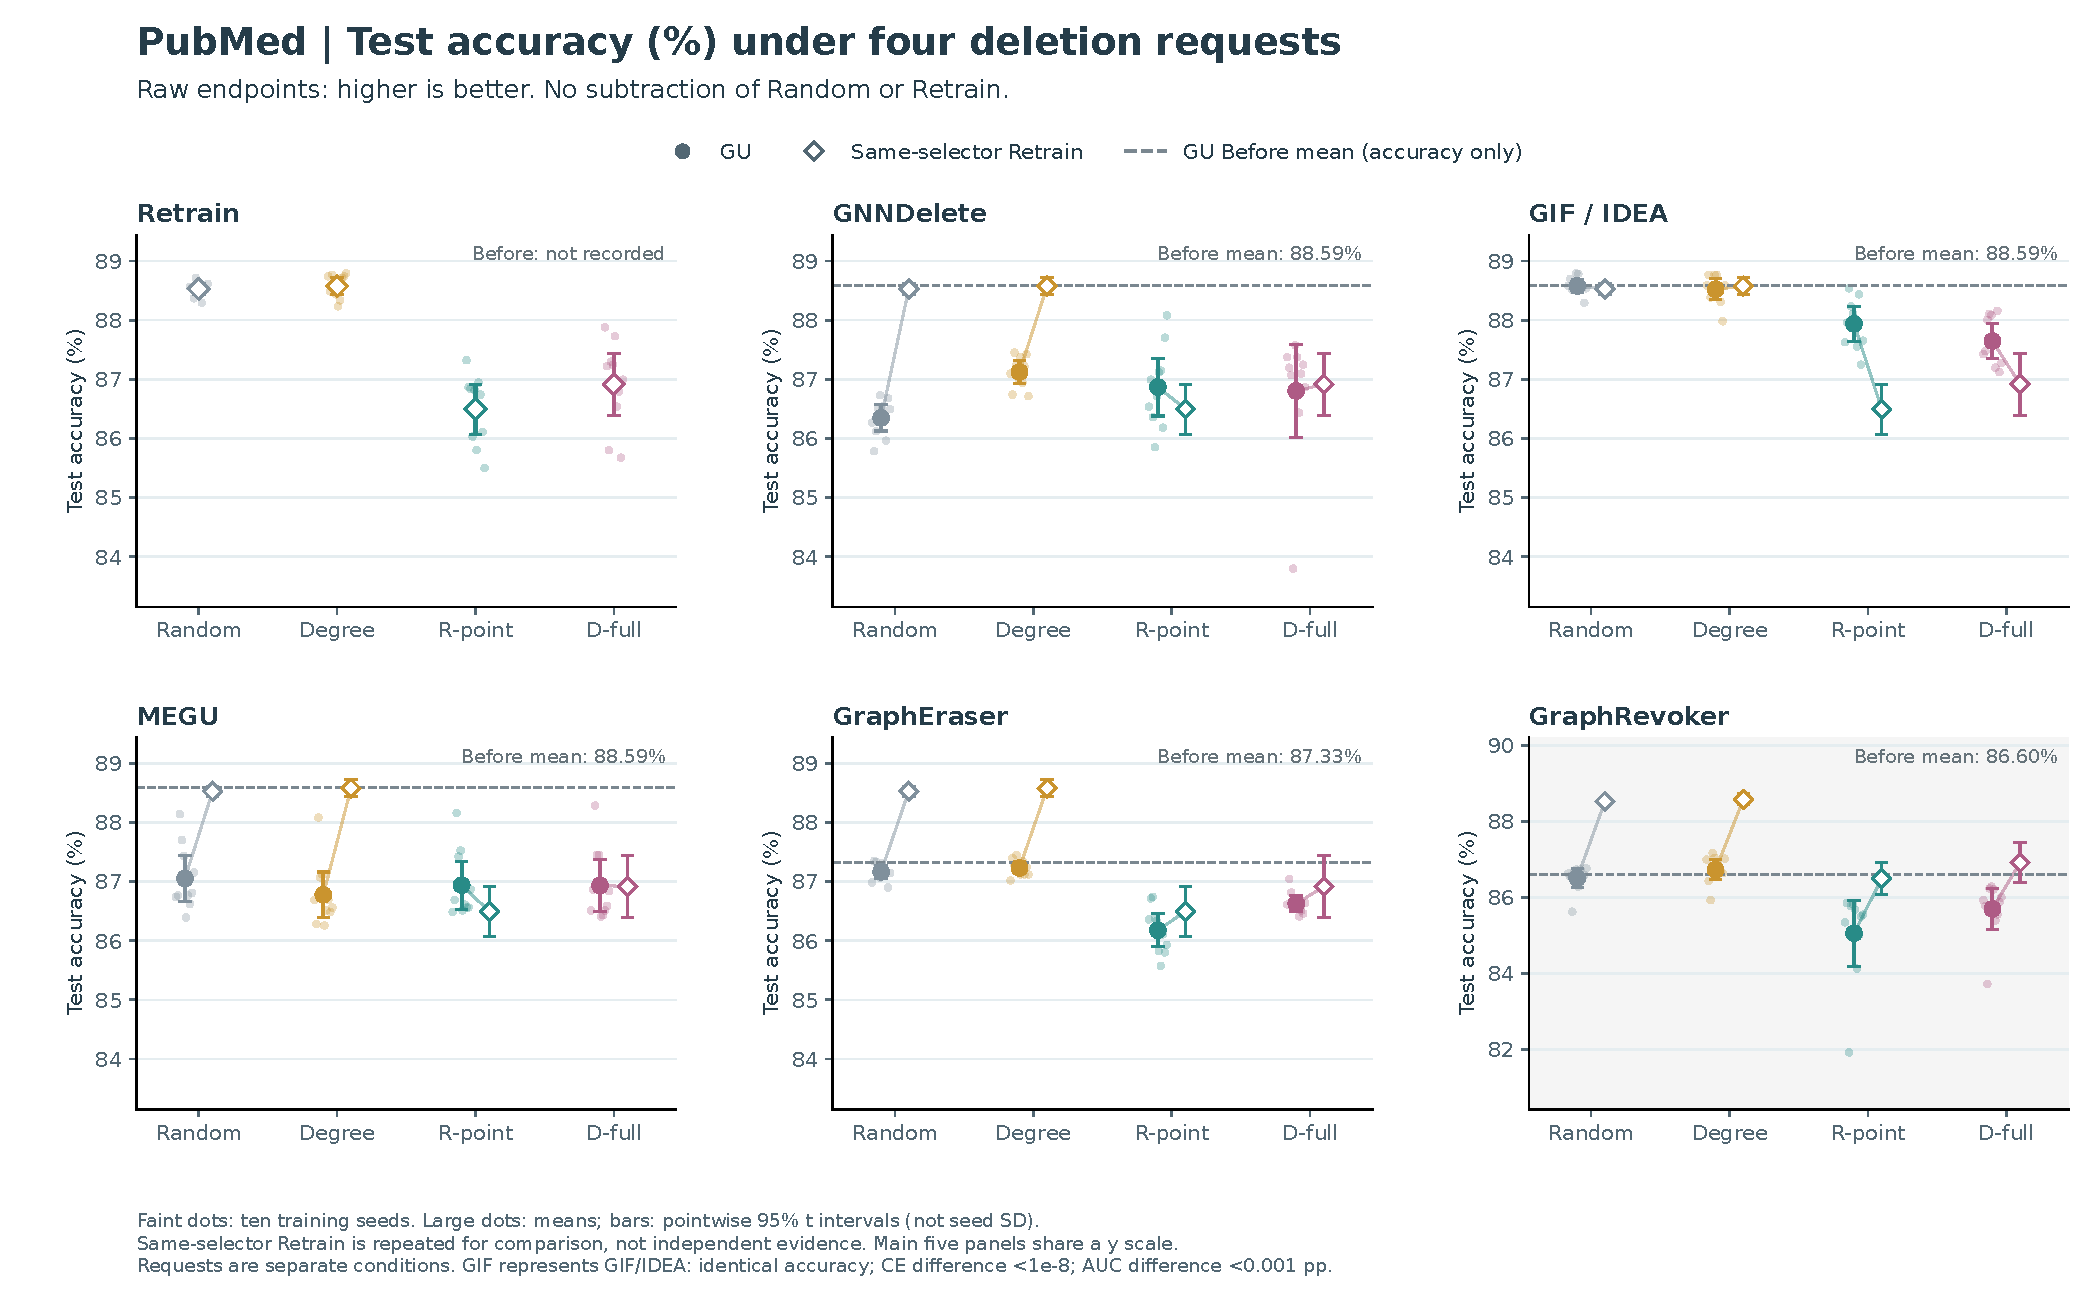
\includegraphics[width=\textwidth]{figures/pubmed_request_patterns.pdf}
  \caption{Request-dependent accuracy patterns on PubMed (EXP-079/e79r5; GCN selection, 10\% deletion). Each panel compares Random, Degree, R-point, and D-full. Filled circles show GU; open diamonds show same-request full-graph GCN retraining; dashed lines mark the GU's own pre-deletion mean. Pale dots are ten training-seed values and bars are pointwise 95\% $t$ intervals of the mean, with Random draws averaged within seed. The first five panels share a scale; the gray GraphRevoker panel uses its own scale and the archived GPA+optimal implementation. GIF/IDEA share a panel because their accuracy values coincide. Repeated retraining endpoints are the same reference, not independent evidence.}
  \Description{Six panels show raw test accuracy under four deletion requests. Retraining groups Random and Degree above the two IF requests. GraphEraser broadly preserves that grouping, GIF and IDEA reverse the two IF means, MEGU has smaller differences, and GNNDelete has its lowest mean under Random.}
  \label{fig:response-pattern-profiles}
\end{figure*}

The short connectors join each GU mean to its same-request retraining mean, rather than indicating a time trajectory. The ten training seeds share a fixed split, candidate pool, and deletion budget. These mean patterns do not establish a stable selector ranking across independent splits or selection sources; overlapping intervals do not establish equivalence. Full-graph GCN retraining is also a different model-family reference for shard ensembles. The archived batch and its implementation scope remain separate from the later revised sharded-method runs.

\subsection{Selector effects persist with method-dependent GU responses}
Figure~\ref{fig:exp080-budget-response} examines selector effects and GU responses across deletion budgets on CiteSeer. The upper-row trajectories show that R-point's utility-damaging effect carries over to several GU methods: as the budget increases, matched Retrain, GNNDelete, GraphEraser, and GraphRevoker exhibit pronounced accuracy declines, while the other selectors generally produce weaker mean accuracy responses. The separation develops along the budget curves. Relative to same-budget Random, R-point reduces GNNDelete, GraphEraser, and GraphRevoker accuracy by 7.61, 11.56, and 16.37 pp at 33\% deletion; these losses reach 10.81, 25.68, and 26.83 pp at 50\%. Thus, the selected requests retain utility effects across multiple GU methods, with different response magnitudes.

The lower row exposes a second response: some GU methods do not reproduce the request-induced utility degradation observed under retraining, and increasingly disagree with that target. From 10\% to 50\% R-point deletion, matched Retrain accuracy falls from 74.92\% to 50.90\%, whereas GIF/IDEA and MEGU stay near 74--75\%. Their prediction disagreement with the matched Retrain rises from 7.41\% to 40.19\% and from 9.21\% to 40.94\%, respectively, with positive paired increases in all three training seeds. At 50\%, their disagreement also exceeds the same-budget Random values by 27.28 and 29.18 pp. High retained accuracy therefore coexists with substantial deviation from the retraining response. We assess this prediction-alignment vulnerability through disagreement, using accuracy to explain how each GU responds to the selected request.

\begin{figure*}[t]
  \centering
  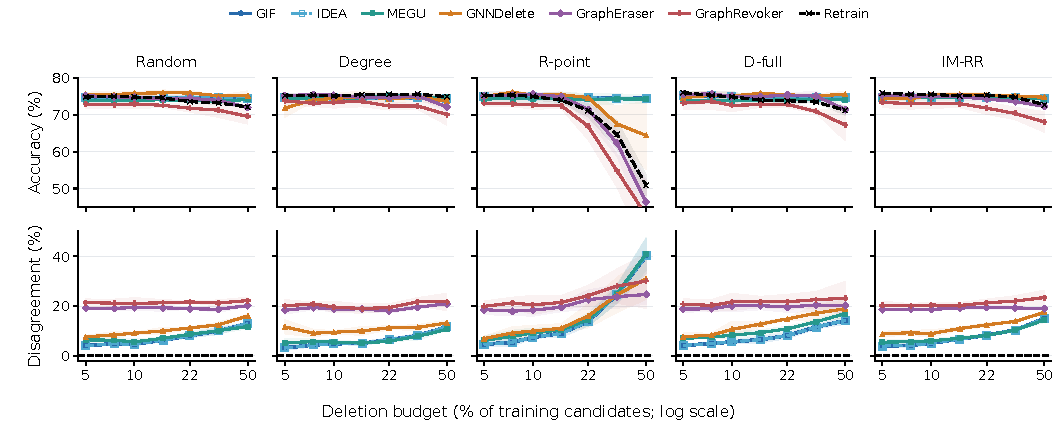
\includegraphics[width=\textwidth]{figures/citeseer_selector_responses.pdf}
  \caption{Selector effects and GU responses on CiteSeer (historical EXP-080). Columns: Random, Degree, R-point, D-full (\texttt{gt\_full}), and IM-RR. Horizontal axes use a logarithmic scale, with deletion budgets labeled in percent. Top: test accuracy, displayed over 45--80\%; curve and SD-band portions outside this range are clipped. Bottom: prediction disagreement with same-request full-graph GCN retraining; the dashed zero line is Retrain's self-comparison. Scales are shared within each row. Curves and shading show three-training-seed means and $\pm1$ sample SD, with IM draws averaged within seed first. GIF and IDEA are separate curves (solid circles / dashed open squares), with coincident outcomes. GraphRevoker uses the archived GPA+optimal implementation; partition-based methods differ in model family from the GCN reference.}
  \Description{Ten line charts in two rows and five selector columns: Random, Degree, R-point, D-full, and IM-RR. Deletion budget is shown on a logarithmic horizontal axis. The upper row shows test accuracy from 45 to 80 percent, clipping values below the displayed range; the lower row shows disagreement with retraining. R-point produces the largest budget-dependent decline in retraining accuracy and increase in GIF, IDEA, and MEGU disagreement. The other four selectors have weaker responses on the same scales.}
  \label{fig:exp080-budget-response}
\end{figure*}

These two layers distinguish the selector's effect on utility from GU deviation relative to the same-request retraining target. The historical CiteSeer curves describe one fixed split and three training seeds. For partition-based methods, the absolute disagreement also includes model-family differences from the full-graph GCN reference. Disagreement diagnoses prediction mismatch; identifying its optimization mechanism or establishing forgetting correctness requires additional evidence.

\subsection{Retraining and GU references expose different sources of change}
In the separate AAGU-032 analysis, the 3000-epoch D-full configurations have lower test accuracy than Degree in 8 of 12 configuration-budget groups on Cora and 10 of 12 on PubMed, but only 4 of 12 on CiteSeer. The mean paired differences (D-full minus Degree) are $-0.277$, $+0.188$, and $-0.922$ pp for Cora, CiteSeer, and PubMed, respectively. This is evidence about the retraining endpoint alone; it cannot be extended to a GU method.

For AAGU-053, Table~\ref{tab:aagu053} decomposes the same-request comparison between the pre-request GNNDelete reference, full retraining, and GNNDelete. Cora and PubMed have positive mean retraining gaps, whereas CiteSeer is near zero. The decomposition preserves the sign and reports distinct descriptive terms by dataset. A near-zero dataset average does not imply request-level equivalence.

\begin{table*}[t]
\centering
\small
\caption{AAGU-053 same-request GNNDelete and full-retraining results at a 10\% budget. Values are equal-weight means over 16 requests per dataset. The stored f1 field is test accuracy in this analysis. Utility values are percentages; differences are pp.}
\label{tab:aagu053}
\begin{tabular}{lrrrrrr}
\toprule
Dataset & $U_0$ & GU & Retrain & $U_0-U_M$ & $U_0-U_R$ & $U_R-U_M$ \\
\midrule
Cora & 90.22 & 70.64 & 89.67 & $+19.580$ & $+0.554$ & $+19.027$ \\
CiteSeer & 74.47 & 74.64 & 74.81 & $-0.169$ & $-0.338$ & $+0.169$ \\
PubMed & 88.56 & 85.80 & 88.48 & $+2.764$ & $+0.087$ & $+2.677$ \\
\bottomrule
\end{tabular}
\end{table*}

The current AAGU-053 update-detection AUC is 0.587, 0.731, and 0.509 for Cora, CiteSeer, and PubMed, respectively. It uses deleted nodes as positives, test nodes as negatives, and prediction-probability change as the score. We report it only as the implemented update-detection diagnostic; it is not a general membership-inference or privacy guarantee.
